\documentclass[./../main_file.tex]{subfiles}

\begin{document}
	Trong phần này, nhóm sẽ giới thiệu một ứng dụng mẫu và các bước để thực hiện ca kiểm thử Selenium trên ứng dụng đó.
	
	\subsection{Hệ thống học trực tuyến Remind Clone}
	
	Ứng dụng được nhóm lựa chọn để thực hiện kiểm thử là hệ thống học trực tuyến Remind Clone. Đây là phần mềm hỗ trợ giáo viên, học sinh, phụ huynh trong việc giảng dạy, học tập và những công việc liên quan đến giáo dục. 
	
	Giáo viên sẽ sử dụng nền tảng này để tạo lớp học và thêm học sinh vào lớp học của mình. Tại đây, giáo viên sẽ có thể nhắn tin, đăng thông báo và chia sẻ tài liệu cho học sinh trong lớp. Ngược lại, học sinh có thể trò chuyện với nhau và với giáo viên của mình. Bằng việc chia người dùng vào từng lớp học riêng biệt, mỗi giáo viên có thể quản lý lớp học của mình hiệu quả hơn. Họ cũng có thể đưa ra một số cài đặt đặc biệt cho lớp mình đang dạy để giúp việc quản lý trở nên dễ dàng hơn.
	
	\begin{figure}[H]
		\centering
		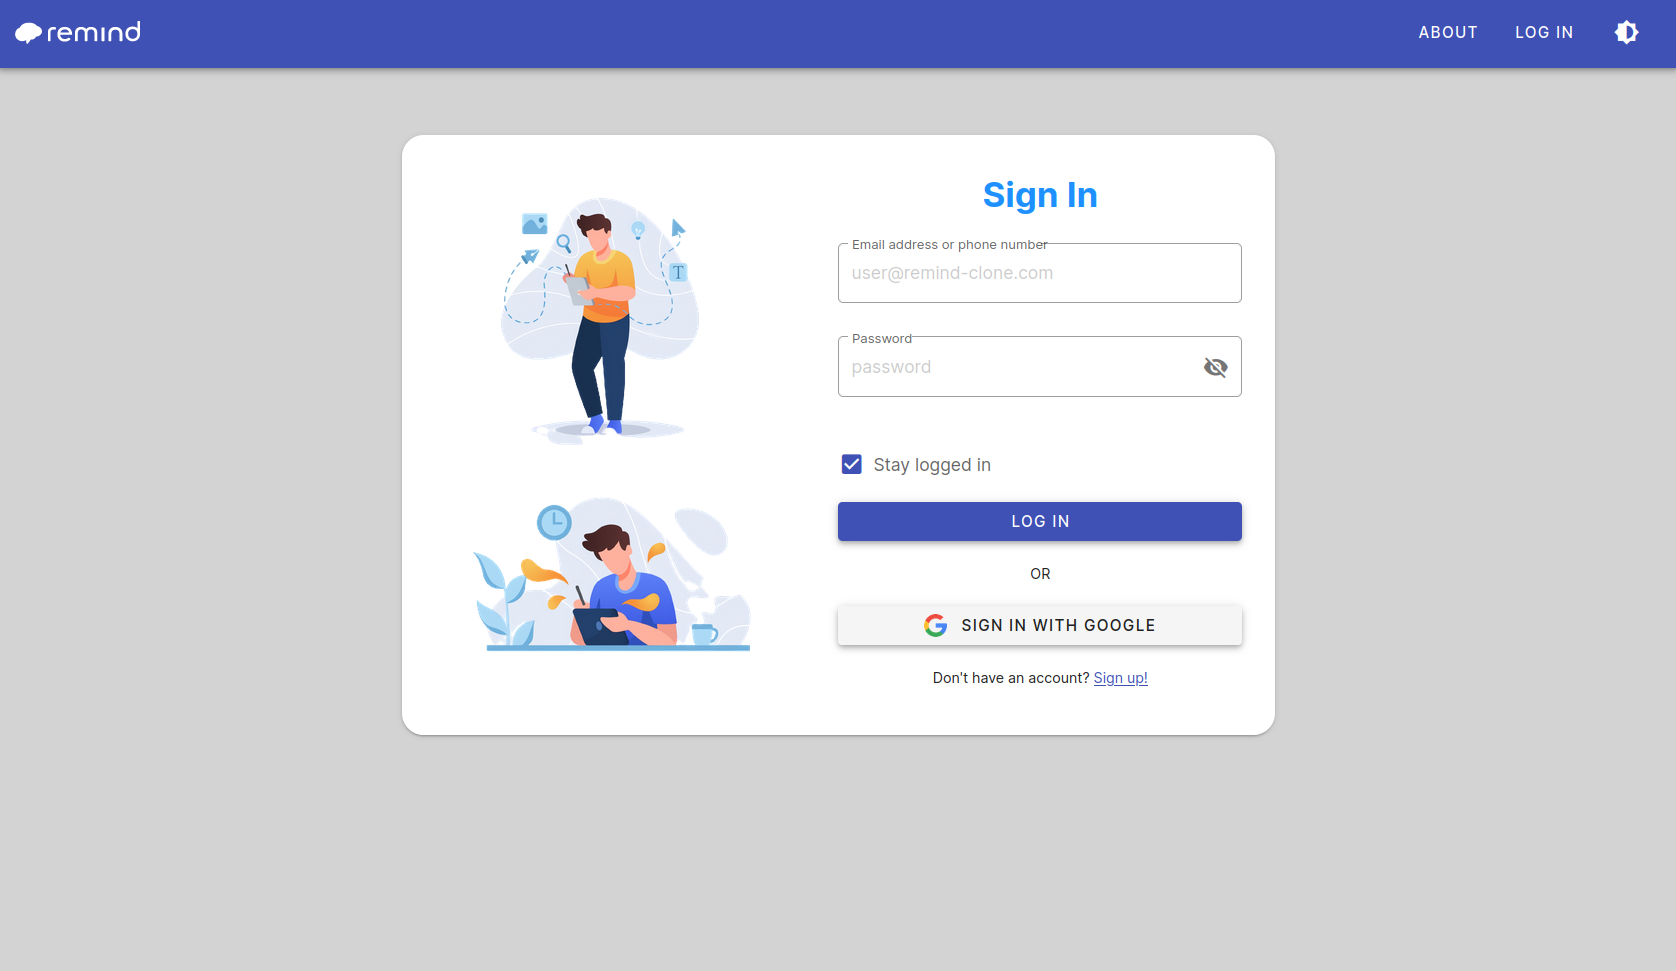
\includegraphics[width=\linewidth]{./images/image4.png}
		\caption{Màn hình đăng nhập}
	\end{figure}

	\begin{figure}\centering
		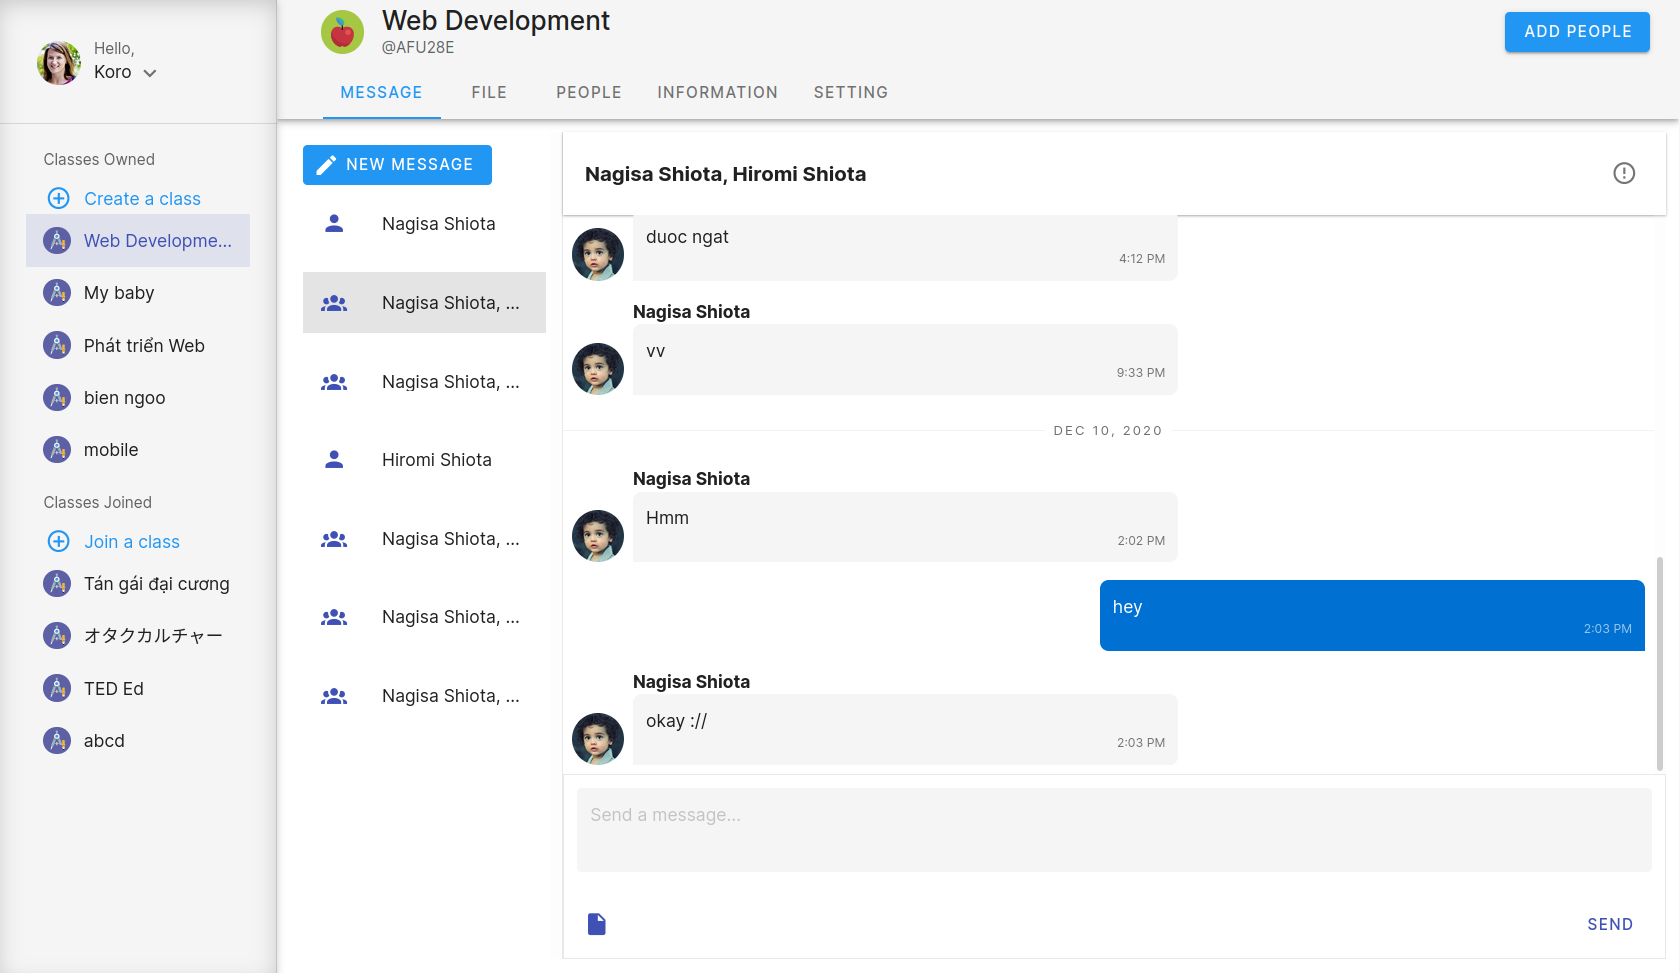
\includegraphics[width=\linewidth]{./images/image2.png}
		\caption{Màn hình chính}
	\end{figure}
	
	\subsection{Phân tích vấn đề}
	
	Trong bước này, nhóm thực hiện phân tích yêu cầu của chương trình. Hệ thống học trực tuyến Remind Clone có những chức năng chính sau:
	
	\begin{itemize}
		\item Đăng nhập và đăng ký
		\item Tạo và gia nhập lớp học
		\item Xem và gửi tin nhắn
		\item Chia sẻ tài liệu
	\end{itemize}

	Khi đã xác định được danh sách chức năng, nhóm sẽ xác định các giao diện và thành phần tương ứng để thực hiện những chức năng đó. Sau khi hoàn thành bước phân tích vấn đề, nhóm sẽ chuyển sang bước tiếp theo, đó là viết ca kiểm thử.
	
	\subsection{Viết ca kiểm thử}
	
	Một ca kiểm thử có nhiệm vụ thực hiện một chức năng cụ thể thông qua việc tương tác với các thành phần giao diện. Thông qua đó, ca kiểm thử có thể xác định tính đúng đắn của hệ thống. Để viết ra các ca kiểm thử cụ thể, Selenium cung cấp cho người dùng hai công cụ là Selenium IDE và Selenium WebDriver. Hai công cụ này phục vụ mục đích tương tự nhau nhưng trong đó, WebDriver đem lại hiệu năng cao hơn cũng như cho phép tùy chỉnh ca kiểm thử dễ dàng hơn. Hơn nữa, WebDriver hỗ trợ nhiều ngôn ngữ lập trình phổ biến, khiến việc viết ca kiểm thử trở nên đơn giản hơn. Vì vậy, nhóm chọn WebDriver để thực hiện việc kiểm thử. Ngoài ra, nhóm cũng sử dụng framework JUnit của Java để so sánh giá trị trả về và sinh báo cáo kết quả kiểm thử.
	
	Ca kiểm thử sẽ được viết theo mẫu thiết kế Page Object Models. Theo mẫu thiết kế này, mỗi trang giao diện cần kiểm thử sẽ được đóng gói thành một class. Các ca kiểm thử thay vì tương tác trực tiếp với giao diện qua WebDriver thì sẽ dựa vào các class này để thực hiện thao tác và lấy các giá trị cần thiết ra để so sánh. Bằng cách này, mã nguồn sẽ có thể tái sử dụng và bảo trì dễ dàng hơn do toàn bộ thao tác liên quan đến giao diện đều được đóng gói. Ngoài ra, các ca kiểm thử sẽ đều kế thừa lớp AbstractTest. Lớp này sẽ khởi tạo đối tượng WebDriver và thực hiện đóng trình duyệt khi ca kiểm thử kết thúc. Cấu trúc file nhóm sử dụng có dạng như sau:
	
	\dirtree{%
		.1 test/.
		.2 AbstractTest.java .
		.2 FileSharingTest.java .
		.2 LoginTest.java .
		.2 page/ .
		.3 FileListPage.java .
		.3 HomePage.java .
		.3 LoginPage.java .
		.3 RegisterPage.java .
		.3 SendMessagePage.java .
		.2 PropertyReader.java .
		.2 RegisterTest.java .
		.2 SendMessageTest.java .
	}

	\subsubsection{Ca kiểm thử cho màn hình đăng nhập}
	
	Màn hình đăng nhập có 3 thành phần chính: input cho email, input cho password và nút đăng nhập. Ca kiểm thử sử dụng một tài khoản có sẵn trong hệ thống để kiểm tra xem người dùng có được đưa tới trang chủ sau khi đăng nhập thành công hay không.
	
	\begin{lstlisting}[language=Java, caption=LoginPage.java]
		import org.openqa.selenium.By;
		import org.openqa.selenium.WebDriver;
		import org.openqa.selenium.WebElement;
		import org.openqa.selenium.support.ui.ExpectedConditions;
		import org.openqa.selenium.support.ui.WebDriverWait;
		
		public class LoginPage {
			protected WebDriver driver;
			
			private By emailBy = By.id("txtEmail");
			private By passwordBy = By.id("txtPassword");
			private By loginBtnBy = By.id("btnSignIn");
			private By formTitleBy = By.className("titleSignin");
			
			public LoginPage(WebDriver driver) {
				this.driver = driver;
				
				new WebDriverWait(driver, 2).until(ExpectedConditions.presenceOfElementLocated(formTitleBy));
			}
			
			public HomePage attemptLogin(String email, String password) {
				WebElement loginInput = driver.findElement(emailBy);
				loginInput.sendKeys(email);
				WebElement passwordInput = driver.findElement(passwordBy);
				passwordInput.sendKeys(password);
				WebElement loginBtn = driver.findElement(loginBtnBy);
				loginBtn.click();
				
				return new HomePage(driver);
			}
		}
	\end{lstlisting}

	\begin{lstlisting}[language=Java,caption=Ca kiểm thử đúng email và mật khẩu]
		@Test
		public void loginWithCorrectInfo() {
			LoginPage loginPage = new LoginPage(driver);
			loginPage.attemptLogin(EMAIL, PASSWORD);
		}
	\end{lstlisting}

	Ngoài ra, trường hợp email hoặc mật khẩu sai cũng được kiểm thử để đảm bảo tính bảo mật của hệ thống.
	
	\begin{lstlisting}[language=Java,caption=Ca kiểm thử sai thông tin đăng nhập]
		@Test
		public void loginWithIncorrectUsername() {
			LoginPage loginPage = new LoginPage(driver);
			assertThrows("User failed to login", Exception.class, () -> loginPage.attemptLogin(WRONG_EMAIL, PASSWORD));
		}
		
		@Test
		public void loginWithIncorrectPassword() {
			LoginPage loginPage = new LoginPage(driver);
			assertThrows("User failed to login", Exception.class, () -> loginPage.attemptLogin(EMAIL, WRONG_PASSWORD));
		}
	\end{lstlisting}
	
	\subsubsection{Ca kiểm thử cho những chức năng khác}
	
	Việc kiểm thử cũng được thực hiện với chức năng đăng ký, nhóm đã kiểm thử trường hợp người dùng điền đúng thông tin đăng ký và trường hợp email bị trùng nhau.
	
	\begin{lstlisting}[language=Java,caption=Ca kiểm thử chức năng đăng ký]
		@Test
		public void pageLoadCorrectly() {
			String registerTitle = new RegisterPage(driver).getFormTitle();
			assertTrue("Correct Title", registerTitle.equals("Sign Up"));
		}
		
		@Test
		public void registerCorrectly() {
			RegisterPage registerPage = new RegisterPage(driver);
			Random rand = new Random();
			
			int randomId = rand.nextInt(1000);
			
			String newUser = "testuser" + randomId;
			String newEmail = "testuser" + randomId + "@email.com";
			String newPassword = "password";
			
			LoginPage loginPage = registerPage.attemptRegister(newUser, newEmail, newPassword, newPassword);
			loginPage.attemptLogin(newEmail, newPassword);
		}
		
		@Test
		public void registerWithExistingEmail() {
			RegisterPage registerPage = new RegisterPage(driver);
			assertThrows(Exception.class,
			() -> registerPage.attemptRegister("newUser", EXISTING_EMAIL, "password", "password"));
		}
	\end{lstlisting}

	Về chức năng chia sẻ file, nhóm thực hiện kiểm thử tính năng upload file. Một file rỗng có tên ngẫu nhiên sẽ được tạo ra và upload lên server. Sau đó, chương trình sẽ kiểm tra file vừa được upload đã thực sự được upload hay chưa. Bằng cách kiểm tra tên của file đó có tồn tại trong danh sách các file trên server, nếu tồn tại thì ca kiểm thử đó sẽ pass.
	
	\begin{lstlisting}[language=Java,caption=Ca kiểm thử gửi file]
		@Test
		public void pageLoadCorrectly() {
			new HomePage(driver).goToFileListPage();
		}
		
		@Test
		public void uploadFile() {
			FileListPage flPage = new HomePage(driver).goToFileListPage();
			File randomFile = createRandomlyNamedFile();
			flPage.uploadFile(randomFile.getAbsolutePath(), "Test File For You And Me");
			
			// check if the file has been successfully uploaded
			flPage.getFileByName(randomFile.getName(), true);
			randomFile.delete();
		}
	\end{lstlisting}
	
	Với tính năng trò chuyện, nhóm sẽ kiểm thử việc gửi và hiển thị tin nhắn. Ở đầu ca kiểm thử, chương trình sẽ thực hiện đăng nhập và truy cập vào cuộc trò chuyện tại lớp học đầu tiên. Với chức năng hiển thị, chương trình sẽ kiểm tra xem có tồn tại tin nhắn trong cuộc trò chuyện này hay không. Mặt khác, với chức năng gửi tin nhắn, chương trình sẽ gửi một tin nhắn ngẫu nhiên, đợi một khoảng thời gian nhất định và kiểm tra xem tin nhắn gần đây nhất có giống với tin vừa được gửi đi hay không.
	
	\begin{lstlisting}[language=Java,caption=Ca kiểm thử gửi tin nhắn]
		private static void goToFirstClassConvo() {
			new WebDriverWait(driver, 3).until(driver -> driver.findElement(By.className("itemClass")));
			new HomePage(driver).goToFirstClassConvo();
			new WebDriverWait(driver, 3).until(driver -> driver.findElement(By.className("itemMessage")));
		}
		
		@Test
		public void pageLoadCorrectly() {
			new HomePage(driver);
		}
		
		@Test
		public void showMessage() throws Exception {
			goToFirstClassConvo();
		}
		
		@Test
		public void sendMessage() throws Exception {
			goToFirstClassConvo();
			SendMessagePage smPage = new SendMessagePage(driver);
			
			Random rand = new Random();
			int randomId = rand.nextInt(10000);
			String newMessage = "Test Message " + randomId;
			smPage.sendMessage(newMessage);
			
			Thread.sleep(1500);
			
			String lastMessage = smPage.getLastMessage();
			assertTrue(lastMessage.equals(newMessage));
		}
	\end{lstlisting}

	\subsubsection{Kiểm thử trên nhiều nền tảng với Selenium Grid}

	Để có thể kiểm thử trên nhiều trình duyệt ở các phiên bản khác nhau, cũng như kiểm thử ứng dụng web trên các hệ điều hành khác, nhóm sử dụng công cụ Selenium Grid. Grid cho phép chúng ta thực thi ca kiểm thử trên nhiều môi trường khác nhau, giúp giảm thiểu rủi ro phần mềm gặp lỗi trên hệ điều hành hay trình duyệt khác.
	
	\subsection{Thực thi ca kiểm thử}
	
	Để thực thi toàn bộ ca kiểm thử với Maven, người dùng chỉ cần chạy câu lệnh sau trong terminal.
	
	\begin{lstlisting}[caption=Chạy toàn bộ ca kiểm thử]
		mvn test
	\end{lstlisting}
	
	\subsubsection{Kết quả kiểm thử}
	
	Dưới đây là kết quả kiểm thử với 13 ca kiểm thử trong chương trình.
	
	\begin{figure}[H]
		\centering
		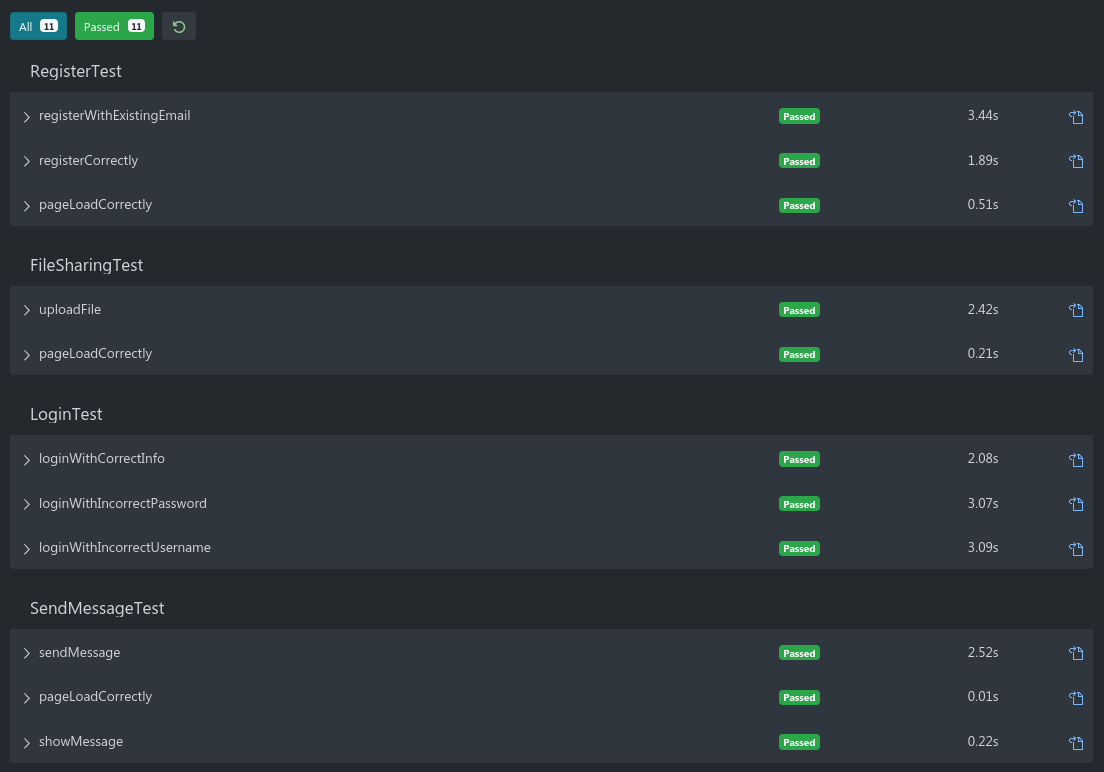
\includegraphics[width=\linewidth]{./images/image6.png}
		\caption{Kết quả kiểm thử}
	\end{figure}
\end{document}